\documentclass[a4paper]{report}

\usepackage[utf8]{inputenc}
\usepackage[margin=1in]{geometry}
\usepackage{color}
\usepackage[draft]{flowfram}
\usepackage[colorlinks]{hyperref}
\usepackage{tubscolors}
\usepackage[a4paper]{tubslogo}
\usepackage[a4paper]{tubstypearea}
% \usepackage{graphicx}

% Use sans-serif font as default font
\renewcommand{\familydefault}{cmss}

% adjust \textheight so that it is an integer multiple of
% \baselineskip
\adjustheight{\textheight}

% set up pagelayout. One column for title page
% two columns for the rest.
\onecolumninarea[1,2]{0.6\textwidth}{\textheight}{0.4\textwidth}{0pt}
\twocolumninarea[>2]{0.6\textwidth}{\textheight}{0.4\textwidth}{0pt}

% Set up dynamic frame on the left. This is where
% the headings will go.

% \newdynamicframe{0.4\textwidth}{\textheight}{0pt}{0pt}[left]

% put the chapter headings in this frame
% \dfchaphead*{left}
% Modify the default style
\renewcommand{\DFchapterstyle}[1]{%
\raggedright\Huge\slshape\MakeUppercase{#1}\par}

\makeatletter

% sets background to 6 specified colors
\newcommand{\tubsSetBackground}[9][1]{%
\hNtoneleft[#1][\tubspage@borderwidth]{8}{\paperwidth-\tubspage@borderwidth}%
% {\textwidth}{tuWhite}{lborder}%
{1\TPVertModule}{#9}{bg1}%
{2\TPVertModule}{#8}{bg2}%
{3\TPVertModule}{#7}{bg3}%
{4\TPVertModule}{#6}{bg4}%
{5\TPVertModule}{#5}{bg5}%
{6\TPVertModule}{#4}{bg6}%
{7\TPVertModule}{#3}{bg7}%
{8\TPVertModule}{#2}{bg8}%
% left white border
\vNtonetop[all]{1}{\paperheight}{\tubspage@borderwidth}{tuWhite}{lborder}
}


% params:
% 1 (opt) - pages to set color for
% 2       - color of first element
% 3       - color of second element
% ...
% 9       - color of last element
\tubsSetBackground[1]%
  {tuBlueDark80}
  {tuBlueDark60}
  {tuBlue}
  {tuBlue80}
  {tuBlue60}
  {tuBlueLight}
  {tuBlueLight80}
  {tuBlueLight60}

% logo
% make a static frame for the logo
% note: small white blank after logo remains...
\newstaticframe[1]{\tulogoWidth}{\tulogoHeight}%
  {-2\tubspage@borderwidth}{-\tubspage@borderwidth+\textheight-0.25\tulogoHeight}[logo]
\setstaticcontents*{logo}{\tubslogo}
\setstaticframe*{logo}{backcolor=tuRed}


\newdynamicframe[1]{\textwidth}{\TPVertModule}{0pt}{0pt}[author]

\setdynamiccontents*{author}{%
  \Huge Enrico Jörns
}

\newdynamicframe[1]{\textwidth}{\TPVertModule}{0pt}{5\TPVertModule}[title]

\setdynamiccontents*{title}{%
  \Huge This Is My Title
}

\newdynamicframe[1]{\textwidth}{15\TPVertModule}{-\tubspage@borderwidth}{20\TPVertModule}[image]

\setdynamiccontents*{image}{%
  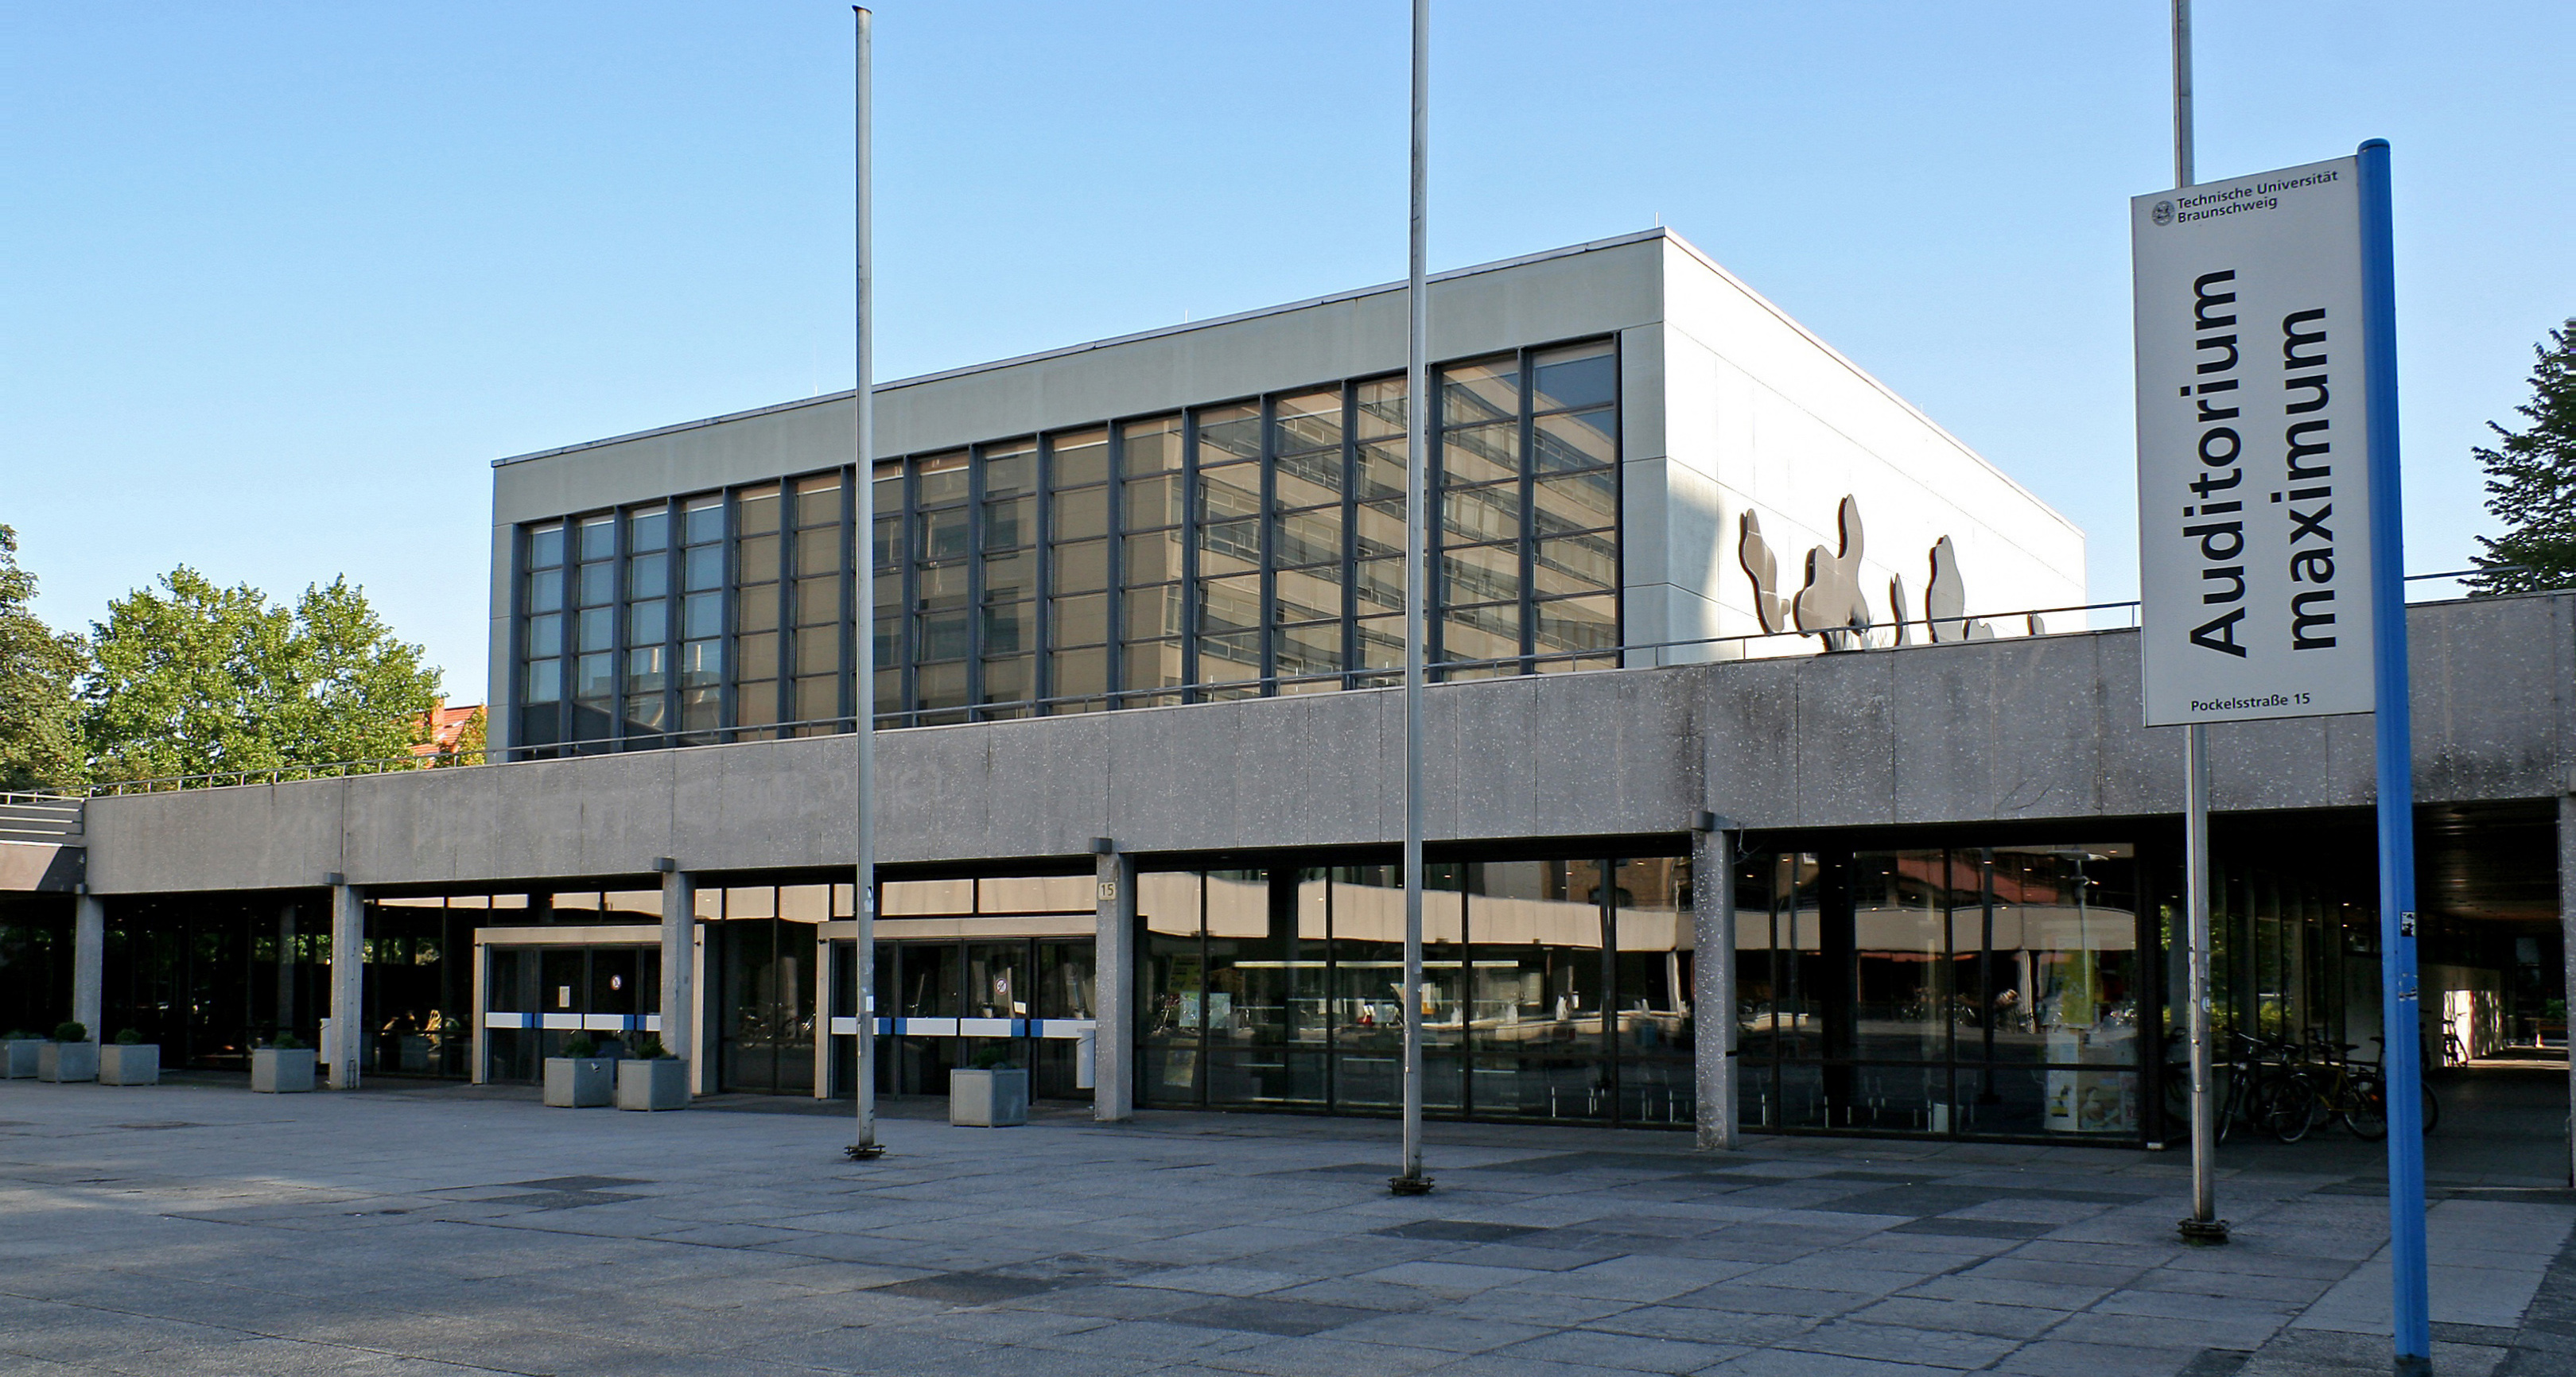
\includegraphics[width=\textwidth+2\tubspage@borderwidth]{../../beamer/doc/titlepicture.jpg}
}

\makeatother
% Make a border along the top of each page
% \vtwotonetop{12cm}{0.6\paperwidth}{[cmyk]{0.65,0.13,0,0}}{topleft}%
% {0.4\paperwidth}{[cmyk]{0.94,0.54,0,0}}{topright}



% empty page style, because I am going to make my own
\pagestyle{empty}

% Each new chapter sets \thispagestyle{\chapterfirstpagestyle}, change this empty as well
\renewcommand{\chapterfirstpagestyle}{empty} 

% % Now make a frame in which to put my own customized footer
% \newdynamicframe[>1]{\textwidth}{\headheight}{0pt}{-\footskip}[footer]
% 
% % set the contents of the frame:
% \setdynamiccontents*{footer}{%
% School of Computing Sciences, University of East Anglia\hfill
% http://www.cmp.uea.ac.uk/\hfill
% page \thepage\ of \pageref*{lastpage}}


\newcommand{\env}[1]{\texttt{#1}}
\newcommand{\cmdname}[1]{\texttt{\symbol{92}#1}}
\newcommand{\meta}[1]{\textnormal{\textless\textit{#1}\textgreater}}

\begin{document}



{\noindent
\slshape\Huge\MakeUppercase{A Sample Brochure}\par
\vskip0.5in
\noindent\large\MakeUppercase{Nicola Talbot}\\
}


\chapter{Introduction}

The \textsl{flowfram} package is designed to enable you to create
frames in a document such that the 
contents of the \env{document} environment flow from one 
frame to the next in the order that they were defined.  
This is useful for creating posters
or magazines or any other form of document that does not 
conform to the standard one or two column layout.

This is a modified version of the manual for the \textsl{flowfram} package.
It is intended to illustrated what can be done. See the full 
manual (ffuserguide.pdf) for
a comprehensive description, as some parts of this document
may now be out of date.
If the columns are very narrow, it may be better to
use \cmdname{raggedright}, otherwise \TeX\ may have a
problem working out the line breaks.

This is column~\thedisplayedframe.

The main type of frame is the flow frame. This is described on
column~\ref{flow:flowframe} on page~\pageref{flow:flowframe}.
The order used to draw the contents of each frame on the page
is described in column~\ref{flow:stacking} on 
page~\pageref{flow:stacking}. Floats are describe in 
column~\ref{flow:floats} on page~\pageref{flow:floats}.

\chapter{Setting up Frames}

This is column~\thedisplayedframe.

The \textsl{flowfram} package provides three types of frame:
{flow frames}, {static 
frames} and {dynamic frames}.

\section*{Flow Frames}

\labelflow{flow:flowframe}
The flow frame is the principle type of frame.
The text of the \env{document} environment will flow from 
one frame to the next in order of definition. Each 
flow frame has an associated width, height, 
position on the page, and optionally a border.

It is recommended that all the flow frames in a document
have the same width, otherwise problems may occur
when a paragraph spans to flow frames of unequal
widths. This is because \TeX's output routine does not
register the change in \cmdname{hsize} until it reaches
a paragraph break. If it is absolutely necessary for 
flow frames to have unequal widths, judicious use of
\cmdname{framebreak} is required.

\section*{Static Frames}

A static frame is a rectangular area in which text neither
flows into, nor flows out of.  The contents must be set
explicitly, and once set, the contents of the static frame will
remain the same on each page until it is explicitly 
changed.  Thus, a static frame can be used, for example, to make 
a company logo appear in the same place on every page.

\section*{Dynamic Frames}

A dynamic frame is similar to a static frame, but its contents
are re-typeset on each page. (A static frame stores its 
contents in a savebox, whereas a dynamic frame stores its
contents in a macro).

This is column~\thedisplayedframe.

\chapter{Frame Attributes}
\label{sec:modattr}

Once you have defined the {flow frames}, {static frames} and 
{dynamic frames}, their attributes can be changed. 
The three types of frame mostly have the 
same set of attributes, but some are specific to a certain type.
The available attributes are as follows
(\textsuperscript{\textbf{F}} indicates the key is
only available for {flow frames}, 
\textsuperscript{\textbf{S}} indicates the key is only available 
for {static frames}
and \textsuperscript{\textbf{D}} indicates the key
is only available for {dynamic frames}):

\begin{description}
\item[width=\meta{length}]\mbox{}\par  The width of the frame.

\item[height=\meta{length}]\mbox{}\par The height of the frame.

\item[x=\meta{length}]\mbox{}\par The x-coordinate of the frame.

\item[y=\meta{length}]\mbox{}\par The y-coordinate of the frame.

\item[border=\meta{style}]\mbox{}\par The style of the border around the 
frame, this can take the values: \texttt{none} (no border),
\texttt{plain} (plain border) or the name of a \LaTeX\ 
frame making command without the preceding backslash. 
The value \texttt{fbox} is equivalent to \texttt{plain}.

\item[offset=\meta{offset}]\mbox{}\par The border offset, if it is a 
user-defined border.  This is the distance from the outer
edge of the left hand border to the left edge of the
bounding box of the text inside the border.  The \textsl{flowfram}
package is able to compute the border for 
known frame making commands. 
If you define your own frame making command, you may need to 
specify the offset explicitly, or the frames 
may end up shifted to the right or left.

\item[bordercolor=\meta{colour}]\mbox{}\par The colour of the border
if you are using a standard frame making command.
The colour can either be specified as, e.g.\ \texttt{green},
or including the colour model, for example 
\verb/[rgb]{0,1,0}/.

\item[textcolor=\meta{colour}]\mbox{}\par The text colour for that 
frame. Again, the colour can either be specified as, 
e.g.\ \texttt{green}, or including the colour model, 
for example \verb/[rgb]{0,1,0}/.

\item[pages=\meta{page list}]\mbox{}\par The {list of 
pages} for which the frame
should appear. This can either have the values: \texttt{all},
\texttt{even}, \texttt{odd} or \texttt{none} (the latter 
removes the frame from that point on---useful if you
have multiple pages with the same number), or it can be a 
comma-separated list of single pages, or 
{page ranges}.

\item[margin=\meta{side}\textsuperscript{F}]\mbox{}\par The side of
the flow frame that its corresponding margin should go on. This
can take the values \texttt{left} or \texttt{right}.

\item[clear=\meta{boolean}\textsuperscript{S}] If this value
is set, the static frame will be cleared at the start of the
next page.

\item[style=\meta{cmd}\textsuperscript{D}]\mbox{}\par This should be
the name of a command \emph{without} the preceding backslash, 
to be applied to the contents of the specified dynamic frame. 
The command may either be a declaration, for example \verb/style=large/
which will set the contents of all the dynamic frames in a
large font, or it can be a command that takes a single argument,
for example \verb/style=textbf/
which will make the text for all the dynamic frames come out in 
bold.  To unset a style, do \verb/style=none/.

\end{description}

\chapter{Miscellaneous}

\section*{Page Layout}

The \textsl{flowfram} package has the package option \texttt{draft}
which will draw the {bounding boxes} for
each frame defined.  At the bottom right of each
bounding box (except for the bounding box denoting the 
typeblock), a marker will be shown to indictate the type
of frame, its IDN and its IDL.

You can see the layout for the current page (irrespective of
whether or not the \texttt{draft} option has been set) using
the command:\newline 
\cmdname{flowframeshowlayout}

The headers and footers will appear as usual (but will not
be shown in draft mode), according to the format given by 
\cmdname{pagestyle}.

\section*{Frame Stacking Order}

\labelflow{flow:stacking}
The material on each page is placed in the following order:
\begin{enumerate}
\item Each static frame defined for that page in ascending
order of IDN.

\item Each flow frame defined for that page in ascending
order of IDN.

\item Each dynamic frame defined for that page in ascending
order of IDN.

\item {Bounding boxes} if the \texttt{draft}
package option has been used.
\end{enumerate}

This ordering can be used to determine if you want something
to overlay or underlay everything else on the page. 

\section*{Prematurely Ending a Flow Frame}

You can force text to move immediately to the next defined
flow frame using one of the standard \LaTeX\ page breaking commands
which  work in an analogous way to the way they
work in standard two column mode. 

The command \cmdname{framebreak} is provided for situations
where a paragraph spans two flow frames
of different widths, as \TeX's output routine does not 
adjust to the new value of \cmdname{hsize} until the last 
paragraph of the previous frame has ended. As a 
result, the end of the paragraph at the beginning of the new
flow frame retains the width of the previous flow frame.

If you want to start a new page, rather than simply move to the 
next frame, use the command\newline
\cmdname{finishthispage}.

\section*{Floats}

\labelflow{flow:floats}
Since floats (such as figures and tables) can only go in 
{flow frames}, this package provides
the additional environments: 
\env{staticfigure} and  
\env{statictable} which can be used in static frames
and dynamic frames. Unlike their \env{figure} and
\env{table} counterparts, they are fixed in place, and
so do not take an optional placement specifier. The 
\cmdname{caption} and \cmdname{label} commands can 
be used within \env{staticfigure} and \env{statictable} as
usual.

The standard \env{figure} and \env{table} commands will 
behave as usual in the flow frames, but their starred versions,
\env{figure*} and \env{table*} behave no differently
from \env{figure} and \env{table}.

\section*{Global Values}

The following macros can be changed using\linebreak \cmdname{renewcommand}:

\begin{itemize}
\item \cmdname{setffdraftcolor} 

This sets the colour of the bounding box
when it is displayed in draft mode.

\item 
\cmdname{setffdrafttypeblockcolor} 

This sets the colour of
the bounding box of the typeblock when it is displayed
in draft mode.

\item \cmdname{fflabelfont}

This sets the font size for the bounding box markers in 
draft mode.

\end{itemize}

The following are lengths, which can be changed using
\cmdname{setlength}:

\begin{itemize}
\item \cmdname{fflabelsep}

This is the distance from the right hand side of the
bounding box at which to place the bounding box marker.

\item \cmdname{flowframesep}

This is the gap between the text of the frame and
its border, for the standard border types. 

\item \cmdname{flowframerule}

This is the width of the frame's border, if using
a border given by a frame making command that uses \cmdname{fboxsep}
to set its border width.

\item \cmdname{columnsep}

This is the horizontal distance between flow frames when using one of the
\cmdname{Ncolumn} type of commands

\item \cmdname{vcolumnsep}

This is the vertical distance between the flow frames and the static or
dynamic frame when using one of the \cmdname{Ncolumntop} type of commands.
\end{itemize}

\label{lastpage}
\end{document}
